\chapter{Concepto probabilístico de anomalía}
\label{chapter:anomalia_probabilidad}

Tras la introducción dada de estadística multivariante ya tenemos los conceptos necesarios para dar la definición alternativa de anomalía basada en probabilidades. Esta definición cabe decir que no es alternativa a la basada en distancias, si no complementaria.

En primer lugar cabe decir que esta definición, al igual que el criterio ya explicado no engloba todas las anomalías y por tanto es algo difícil de medir. Esta definición hace referencia, según mi criterio, a un enfoque que se debe poner junto a la definición basada en distancias y no en contraposición. El objetivo de esta definición es obtener anomalías que no son triviales y se esconden entre los datos.

La base del razonamiento de este tipo de anomalías surge del hecho de que un objeto puede ser anómalo en un subespacio concreto de los datos, pero no en el espacio total. Vamos a introducir un ejemplo para visualizar un tipo de anomalía que encaje con esta definición.

Veamos la siguiente figura:

\begin{figure}[H]
	\centering
	\label{ejemplo_anomalia_probabilidad}
	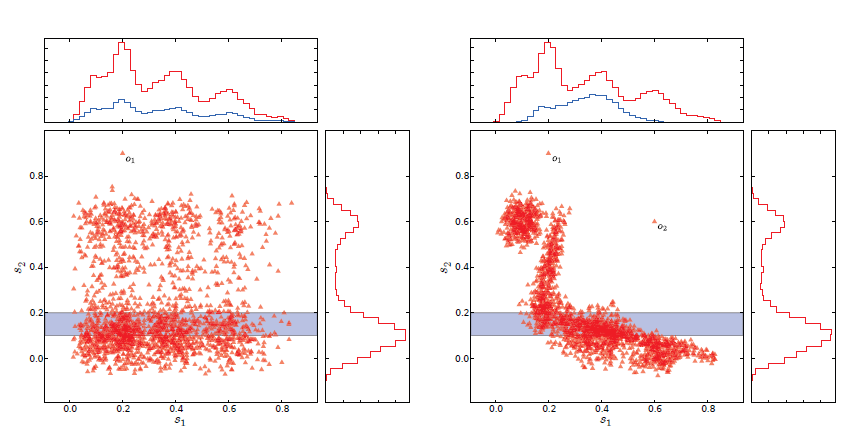
\includegraphics[scale=0.6]{imagenes/ejemplo_anomalia_probabilidad}
	\caption{Ejemplo de anomalía \cite{fabian_keller_hics:_2012}}
\end{figure}

Como se puede observar tenemos dos espacios: el izquierdo no presenta datos correlados y el derecho sí presenta correlación. Podemos ver que en ambos casos se comparte una anomalía etiquetada como $O_1$. Esta anomalía en el caso del espacio no correlado es perfectamente detectable de forma trivial observando las proyecciones de los datos en una dimensión. En cambio en el segundo caso ninguna de las dos anomalías etiquetadas $O_1 , O_2$ son detectables de esta forma trivial, pues si hacemos las proyecciones uno dimensionales ninguno de los dos datos es discordante en dichas proyecciones. Estas anomalías son las que decimos que son no triviales. En cambio si observamos los datos en una proyección de orden superior como la que estamos viendo de dimensión 2 podemos observar claramente que se salen de la correlación de datos que muestra el resto. Es aquí donde podemos ver que en el conjunto de la derecha ninguno de los puntos es una anomalía en las proyecciones de dimensión uno pero sí lo son en la proyección de dimensión 2.

Vamos por tanto a definir más formalmente este concepto especial de anomalía. Necesitamos introducir en primer lugar un poco de notación.

Partimos de un conjunto de datos $X = \{ x_1 , ... , x_n \}$ de $n$ objetos cada uno tomando $d$ valores, es decir, $x_i = (x_{s_1} , ... , x_{s_d}) \in \mathbb{R}^d$. Notamos un subespacio del conjunto de valores como:

$$S = \{ s_i | s_i \in \{ s_1 , ... , s_d \} \ con \ i\in \Delta \}$$

Dado un subespacio $S = \{ s_1 , ... , s_p \}$ notamos la proyección de los objetos del conjunto de datos como $X_{S} = \{ x_{s_1} , ... , x_{s_p} \}$.

Esta proyección está distribuida según una distribución conjunta desconocida de $S$:

$$p_{s_1 , ... , s_p} (x_{s_1} , ... , x_{s_p})$$

Notamos la distribución marginal asociada al atributo $s_i$ como:

$$p_{s_i}(x_{s_i})$$

\begin{definicion}
	Decimos que un subespacio $S$ es un espacio incorrelado si y sólo si:
	
	$$p_{s_1 , ... , s_p}(x_{s_1} , ... , x_{s_p}) = \prod_{i=1}^{p}p_{s_i}(x_{s_i})$$
\end{definicion}

Por tanto si estamos bajo la suposición de un espacio incorrelado podemos decir que la densidad esperada es:

$$p_{esp}(x_{s_1} , ... , x_{s_p}) \equiv \prod_{i=1}^{p}p_{s_i}(x_{s_i})$$

Recordemos que nuestras anomalías no triviales no están en este tipo de subespacios, si no en los correlados. Por tanto vamos a definirlo de la siguiente forma:

\begin{definicion}
	Decimos que un objeto $x_{S}$ es una anomalía no trivial respecto al subespacio $S$ si:
	
	$$p_{s_1 , ... , s_p}(x_{s_1} , ... , x_{s_p}) \ll p_{esp}(x_{s_1} , ... , x_{s_p})$$
	
	Es decir, si la probabilidad esperada es significativamente mayor que la probabilidad conjunta.
\end{definicion}

Por cómo hemos definido los espacios correlados e incorrelados es claro que no podemos tener anomalías en espacios no correlados como es evidente pues la densidad conjunta y esperada serían iguales.

Este concepto como podemos observar no comparte ninguna relación con nuestra definición de anomalías basadas en distancias por lo que es de esperar que si comparamos ambos tipos de anomalías en un conjunto de datos no obtengamos los mismos objetos.